% Capitolul 2: Modele ARMA
% Prezentare academică de calitate Harvard
% Program de licență, Academia de Studii Economice din București

\documentclass[9pt, aspectratio=169, t]{beamer}

% Asigură încadrarea conținutului pe diapozitive
\setbeamersize{text margin left=8mm, text margin right=8mm}

%=============================================================================
% CONFIGURARE TEMĂ ȘI STIL
%=============================================================================
\usetheme{default}
% Utilizăm tema implicită pentru control curat al antetului/subsolului

% Paletă de Culori (potrivită cu PDF-ul Redispatch)
\definecolor{MainBlue}{RGB}{26, 58, 110}
\definecolor{AccentBlue}{RGB}{26, 58, 110}
\definecolor{IDAred}{RGB}{205, 0, 0}
\definecolor{DarkGray}{RGB}{51, 51, 51}
\definecolor{MediumGray}{RGB}{128, 128, 128}
\definecolor{LightGray}{RGB}{248, 248, 248}
\definecolor{VeryLightGray}{RGB}{235, 235, 235}
\definecolor{KeynoteGray}{RGB}{218, 218, 218}
\definecolor{SectionGray}{RGB}{120, 120, 120}
\definecolor{FooterGray}{RGB}{100, 100, 100}
\definecolor{Crimson}{RGB}{220, 53, 69}
\definecolor{Forest}{RGB}{46, 125, 50}
\definecolor{Amber}{RGB}{181, 133, 63}
\definecolor{Orange}{RGB}{230, 126, 34}
\definecolor{Purple}{RGB}{142, 68, 173}

% Fundal gradient (gradient Keynote exact 315°: alb la RGB 218,218,218)
\setbeamertemplate{background}{%
    \begin{tikzpicture}[remember picture, overlay]
        \shade[shading=axis, shading angle=315,
        top color=white, bottom color=KeynoteGray]
        (current page.south west) rectangle (current page.north east);
    \end{tikzpicture}%
}
% Culoare solidă de rezervă pentru compatibilitate
\setbeamercolor{background canvas}{bg=}

\setbeamercolor{palette primary}{bg=MainBlue, fg=white}
\setbeamercolor{palette secondary}{bg=MainBlue!85, fg=white}
\setbeamercolor{palette tertiary}{bg=MainBlue!70, fg=white}
\setbeamercolor{structure}{fg=MainBlue}
\setbeamercolor{title}{fg=IDAred}
\setbeamercolor{frametitle}{fg=IDAred, bg=}
\setbeamercolor{block title}{bg=MainBlue, fg=white}
\setbeamercolor{block body}{bg=VeryLightGray, fg=DarkGray}
\setbeamercolor{block title alerted}{bg=Crimson, fg=white}
\setbeamercolor{block body alerted}{bg=Crimson!8, fg=DarkGray}
\setbeamercolor{block title example}{bg=Forest, fg=white}
\setbeamercolor{block body example}{bg=Forest!8, fg=DarkGray}
\setbeamercolor{item}{fg=MainBlue}

% Culori subsol (suprascriu albastrul temei Madrid)
\setbeamercolor{author in head/foot}{fg=FooterGray, bg=}
\setbeamercolor{title in head/foot}{fg=FooterGray, bg=}
\setbeamercolor{date in head/foot}{fg=FooterGray, bg=}
\setbeamercolor{section in head/foot}{fg=FooterGray, bg=}
\setbeamercolor{subsection in head/foot}{fg=FooterGray, bg=}

% Stiluri marcatori (se aplică peste tot inclusiv în blocuri)
\setbeamertemplate{itemize item}{\color{MainBlue}$\boxdot$}
\setbeamertemplate{itemize subitem}{\color{MainBlue}$\blacktriangleright$}
\setbeamertemplate{itemize subsubitem}{\color{MainBlue}\tiny$\bullet$}
\setbeamertemplate{itemize/enumerate body begin}{\normalsize}
\setbeamertemplate{itemize/enumerate subbody begin}{\normalsize}

% Spațierea elementelor
\setlength{\leftmargini}{1.5em}
\setlength{\leftmarginii}{1.5em}

\setbeamertemplate{navigation symbols}{}

% TOC with bullets
\setbeamertemplate{section in toc}{\color{MainBlue}$\boxdot$\hspace{0.5em}\inserttocsection}

%=============================================================================
% ANTET PERSONALIZAT
%=============================================================================
\setbeamertemplate{headline}{%
    \vskip10pt%
    \hbox to \paperwidth{%
        \hskip0.5cm%
        {\small\color{FooterGray}\renewcommand{\hyperlink}[2]{##2}\insertsectionhead}%
        \hfill%
        \textcolor{FooterGray}{\small\insertframenumber}%
        \hskip0.5cm%
    }%
    \vskip4pt%
    {\color{FooterGray}\hrule height 0.4pt}%
}

%=============================================================================
% SUBSOL PERSONALIZAT
%=============================================================================
\usepackage{fontawesome5}

\setbeamertemplate{footline}{%
    {\color{FooterGray}\hrule height 0.4pt}%
    \vskip4pt%
    \hbox to \paperwidth{%
        \hskip0.5cm%
        \textcolor{FooterGray}{\small Analiza și Prognoza Seriilor de Timp}%
        \hfill%
        \raisebox{-0.1em}{%
            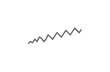
\begin{tikzpicture}[x=0.08em, y=0.08em, line width=0.4pt]
                \draw[FooterGray] (0,3) -- (1,4) -- (2,3.5) -- (3,5) -- (4,4) -- (5,6) -- (6,5.5) -- (7,4) -- (8,5) -- (9,7) -- (10,6) -- (11,5) -- (12,6.5) -- (13,8) -- (14,7) -- (15,6) -- (16,7.5) -- (17,9) -- (18,8) -- (19,7) -- (20,8.5) -- (21,10) -- (22,9) -- (23,8) -- (24,9.5);
            \end{tikzpicture}%
        }%
        \hskip0.5cm%
    }%
    \vskip6pt%
}

%=============================================================================
% PACHETE
%=============================================================================
\usepackage[utf8]{inputenc}
\usepackage[T1]{fontenc}
\usepackage{amsmath, amssymb, amsthm}
\usepackage{mathtools}
\usepackage{bm}
\usepackage{tikz}
\usetikzlibrary{arrows.meta, positioning, shapes, calc, decorations.pathreplacing, shadings}
\usepackage{booktabs}
\usepackage{colortbl}
\usepackage{multirow}
\usepackage{array}
\usepackage{graphicx}
\usepackage{hyperref}
\hypersetup{colorlinks=true, linkcolor=MainBlue, urlcolor=MainBlue}
\graphicspath{{../logos/}{../charts/}}

%=============================================================================
% COMANDA QUANTLET
%=============================================================================
\newcommand{\quantlet}[2]{%
    \begin{tikzpicture}[remember picture, overlay]
        \node[anchor=south east, inner sep=0pt] at ([xshift=-0.5cm, yshift=0.75cm]current page.south east) {%
            \href{#2}{%
                \raisebox{-0.1em}{\includegraphics[height=0.8em]{ql_logo.png}}%
                \textcolor{MainBlue}{\scriptsize\ #1}%
            }%
        };
    \end{tikzpicture}%
}

%=============================================================================
% PAGINĂ DE TITLU PERSONALIZATĂ
%=============================================================================
\defbeamertemplate*{title page}{hybrid}[1][]
{
    \vspace{0.2cm}
    % Rând logo-uri - antet superior (cu linkuri clickabile)
    \begin{center}
        \href{https://www.ase.ro}{\includegraphics[height=1.0cm]{ase_logo.png}}\hspace{0.3cm}%
        \href{https://theida.net}{\includegraphics[height=1.0cm]{ida_logo.png}}\hspace{0.3cm}%
        \href{https://blockchain-research-center.com}{\includegraphics[height=1.0cm]{brc_logo.png}}\hspace{0.3cm}%
        \href{https://www.ai4efin.ase.ro}{\includegraphics[height=1.0cm]{ai4efin_logo.png}}\hspace{0.3cm}%
        \href{https://ipe.ro/new}{\includegraphics[height=1.0cm]{acad_logo.png}}\hspace{0.3cm}%
        \href{https://www.digital-finance-msca.com}{\includegraphics[height=1.0cm]{msca_logo.png}}%
    \end{center}

    \vspace{0.6cm}

    % Titlu principal cu logo-uri Q pe părți (cu linkuri clickabile)
    \begin{center}
        \begin{minipage}{0.1\textwidth}
            \centering
            \href{https://quantlet.com}{\includegraphics[height=1.1cm]{ql_logo.png}}
        \end{minipage}%
        \begin{minipage}{0.78\textwidth}
            \centering
            {\LARGE\bfseries\usebeamercolor[fg]{title}\inserttitle}

            \vspace{0.3cm}

            {\usebeamerfont{subtitle}\usebeamercolor[fg]{title}\insertsubtitle}
        \end{minipage}%
        \begin{minipage}{0.1\textwidth}
            \centering
            \href{https://quantinar.com}{\includegraphics[height=1.1cm]{qr_logo.png}}
        \end{minipage}
    \end{center}

    \vspace{0.6cm}

    % Autori (aliniere la stânga)
    \hspace{0.5cm}{\usebeamerfont{author}\insertauthor}

    \vspace{0.3cm}

    % Institut/Afilieri (aliniere la stânga)
    \hspace{0.5cm}\begin{minipage}[t]{0.9\textwidth}
        \raggedright\small\insertinstitute
    \end{minipage}
}

%=============================================================================
% MEDII PENTRU TEOREME
%=============================================================================
\theoremstyle{definition}
\setbeamertemplate{theorems}[numbered]
\newtheorem{defn}{Definiție}
\newtheorem{thm}{Teoremă}
\newtheorem{prop}{Propoziție}
\newtheorem{rmk}{Observație}

%=============================================================================
% COMENZI PERSONALIZATE
%=============================================================================
\newcommand{\E}{\mathbb{E}}
\newcommand{\Var}{\text{Var}}
\newcommand{\Cov}{\text{Cov}}
\newcommand{\Corr}{\text{Corr}}
\newcommand{\R}{\mathbb{R}}
\newcommand{\N}{\mathbb{N}}
\newcommand{\Z}{\mathbb{Z}}
\newcommand{\B}{\mathbf{B}}
\newcommand{\imark}{\textcolor{MainBlue}{\textbullet}}
\newcommand{\RMSE}{\text{RMSE}}
\newcommand{\MAE}{\text{MAE}}
\newcommand{\MAPE}{\text{MAPE}}

%=============================================================================
% INFORMAȚII TITLU
%=============================================================================
\title[Analiza Seriilor de Timp]{Analiza și Prognoza Seriilor de Timp}
\subtitle{Capitolul 2: Modele ARMA}
\author[D.T. Pele]{Daniel Traian PELE}
\institute{Academia de Studii Economice din București\\
IDA Institute Digital Assets\\
Blockchain Research Center\\
AI4EFin Artificial Intelligence for Energy Finance\\
Academia Română, Institutul de Prognoză Economică\\
MSCA Digital Finance}
\date{}

\begin{document}

% Pagina de titlu (fără antet/subsol)
{
\setbeamertemplate{headline}{}
\setbeamertemplate{footline}{}
\begin{frame}
    \titlepage
\end{frame}
}

%=============================================================================
% CUPRINS
%=============================================================================
\begin{frame}{Structura Cursului}
    \tableofcontents
\end{frame}

%=============================================================================
% MOTIVAȚIE
%=============================================================================
\section{Motivație}

\begin{frame}{Exemplu Motivațional: Procese Staționare}
    \vspace{-0.3cm}
    \begin{center}
        \includegraphics[width=0.92\textwidth, height=0.62\textheight, keepaspectratio]{ch2_motivation_stationary.png}
    \end{center}
    \vspace{-0.2cm}
    {\footnotesize
    \begin{itemize}
        \item \textbf{Procese AR}: Valoarea curentă depinde de valorile trecute --- comportament de revenire la medie
        \item \textbf{Procese MA}: Valoarea curentă depinde de șocurile trecute --- memorie scurtă
        \item \textbf{ARMA}: Combină ambele mecanisme pentru modelare flexibilă
    \end{itemize}
    }
    \quantlet{TSA\_ch2\_motivation}{https://github.com/QuantLet/TSA/tree/main/TSA_ch2_motivation}
\end{frame}

\begin{frame}{Identificarea Modelului prin Tipare ACF}
    \vspace{-0.3cm}
    \begin{center}
        \includegraphics[width=0.95\textwidth, height=0.58\textheight, keepaspectratio]{ch2_motivation_acf.png}
    \end{center}
    \vspace{-0.2cm}
    {\footnotesize
    \begin{exampleblock}{ACF Dezvăluie Structura Modelului}
        \begin{itemize}
            \item Diferite modele ARMA produc tipare ACF distincte
            \item Putem identifica modelul examinând datele!
        \end{itemize}
    \end{exampleblock}
    }
    \quantlet{TSA\_ch2\_motivation}{https://github.com/QuantLet/TSA/tree/main/TSA_ch2_motivation}
\end{frame}

%=============================================================================
% SECȚIUNEA 1: INTRODUCERE ȘI OPERATORUL LAG
%=============================================================================
\section{Introducere și Operatorul Lag}

\begin{frame}{Recapitulare: Staționaritatea}
    \textbf{Din Capitolul 1:} Un proces $\{X_t\}$ este \textbf{slab staționar} dacă:
    \begin{enumerate}
        \item $\E[X_t] = \mu$ (medie constantă)
        \item $\Var(X_t) = \sigma^2 < \infty$ (varianță constantă, finită)
        \item $\Cov(X_t, X_{t+h}) = \gamma(h)$ (covarianța depinde doar de lag-ul $h$)
    \end{enumerate}

    \vspace{0.15cm}
    \textbf{De ce contează staționaritatea pentru ARMA:}
    \begin{itemize}
        \item Modelele ARMA presupun că procesul subiacent este staționar
        \item Datele nestaționare trebuie diferențiate mai întâi (ARIMA)
        \item Staționaritatea asigură parametri stabili ai modelului
    \end{itemize}

    \vspace{0.15cm}
    \textbf{Astăzi:} Construim modele pentru serii de timp staționare folosind valori trecute și erori trecute.
\end{frame}

\begin{frame}{Operatorul Lag (Operatorul de Întârziere)}
    \begin{defn}[Operatorul Lag]
        \textbf{Operatorul lag} $L$ (sau operatorul de întârziere $B$) deplasează o serie de timp înapoi cu o perioadă:
        $$L X_t = X_{t-1}$$
    \end{defn}

    \textbf{Proprietăți:}
    \begin{itemize}
        \item $L^k X_t = X_{t-k}$ (deplasare înapoi cu $k$ perioade)
        \item $L^0 X_t = X_t$ (identitate)
        \item $(1-L)X_t = X_t - X_{t-1} = \Delta X_t$ (prima diferență)
        \item $(1-L)^d X_t = \Delta^d X_t$ (diferența de ordin $d$)
    \end{itemize}

    \vspace{0.15cm}
    \textbf{Polinoame Lag:}
    $$\phi(L) = 1 - \phi_1 L - \phi_2 L^2 - \cdots - \phi_p L^p$$
    $$\theta(L) = 1 + \theta_1 L + \theta_2 L^2 + \cdots + \theta_q L^q$$
    \quantlet{TSA\_ch2\_lag\_operator}{https://github.com/QuantLet/TSA/tree/main/TSA_ch2_lag_operator}
\end{frame}

\begin{frame}{Operatorul Lag: Ilustrație Vizuală}
    \begin{center}
        \includegraphics[width=0.88\textwidth, height=0.65\textheight, keepaspectratio]{lag_operator.png}
    \end{center}

    \vspace{0.2cm}
    \textbf{Observație cheie:} Operatorul lag este fundamentul notației modelelor ARMA
    \quantlet{TSA\_ch2\_lag\_operator}{https://github.com/QuantLet/TSA/tree/main/TSA_ch2_lag_operator}
\end{frame}

\begin{frame}{Procesul de Zgomot Alb}
    \begin{defn}[Zgomot Alb]
        Un proces $\{\varepsilon_t\}$ este \textbf{zgomot alb}, notat $\varepsilon_t \sim WN(0, \sigma^2)$, dacă:
        \begin{enumerate}
            \item $\E[\varepsilon_t] = 0$ pentru toți $t$
            \item $\Var(\varepsilon_t) = \sigma^2$ pentru toți $t$
            \item $\Cov(\varepsilon_t, \varepsilon_s) = 0$ pentru toți $t \neq s$
        \end{enumerate}
    \end{defn}

    \vspace{0.15cm}
    \textbf{Proprietăți:}
    \begin{itemize}
        \item Zgomotul alb este ``blocul de construcție'' al modelelor ARMA
        \item ACF: $\rho(0) = 1$, $\rho(h) = 0$ pentru $h \neq 0$
        \item PACF: același tipar
        \item \textbf{Zgomot alb Gaussian:} adițional $\varepsilon_t \sim N(0, \sigma^2)$
    \end{itemize}

    \vspace{0.15cm}
    \textbf{Notă:} Zgomotul alb \textit{nu} este predictibil --- este pur aleatoriu.
\end{frame}

\begin{frame}{Zgomot Alb: Ilustrare Vizuală}
    \begin{center}
        \includegraphics[width=0.95\textwidth, height=0.52\textheight, keepaspectratio]{ch2_white_noise.png}
    \end{center}
    \vspace{-0.2cm}
    {\footnotesize
    \begin{block}{Caracteristici Cheie}
        \begin{itemize}
            \item \textbf{Stânga}: Seria fluctuează aleatoriu în jurul mediei zero, fără tipare
            \item \textbf{Dreapta}: ACF arată doar un vârf la lag 0; toate celelalte în intervalul de încredere
        \end{itemize}
    \end{block}
    }
    \quantlet{TSA\_ch2\_white\_noise}{https://github.com/QuantLet/TSA/tree/main/TSA_ch2_white_noise}
\end{frame}

%=============================================================================
% SECȚIUNEA 2: MODELE AR
%=============================================================================
\section{Modele Autoregresive (AR)}

\begin{frame}{Modelul AR(1): Definiție}
    \begin{defn}[Proces AR(1)]
        Un \textbf{proces autoregresiv de ordin 1} este:
        $$X_t = c + \phi X_{t-1} + \varepsilon_t$$
        unde $\varepsilon_t \sim WN(0, \sigma^2)$ și $|\phi| < 1$ pentru staționaritate.
    \end{defn}

    \vspace{0.15cm}
    \textbf{Interpretare:}
    \begin{itemize}
        \item $c$: constantă (interceptul)
        \item $\phi$: coeficient autoregresiv --- măsoară persistența
        \item $\varepsilon_t$: inovație (șoc impredictibil)
    \end{itemize}

    \vspace{0.15cm}
    \textbf{Folosind operatorul lag:}
    $$(1 - \phi L)X_t = c + \varepsilon_t$$
    $$\phi(L) X_t = c + \varepsilon_t \quad \text{unde } \phi(L) = 1 - \phi L$$
\end{frame}

\begin{frame}{AR(1): Ilustrație Vizuală}
    \begin{center}
        \includegraphics[width=0.95\textwidth, height=0.52\textheight, keepaspectratio]{ch2_def_ar1.png}
    \end{center}
    \vspace{-0.2cm}
    {\footnotesize
    \begin{itemize}
        \item \textbf{$\phi$ pozitiv}: Fluctuații persistente, revenire graduală la medie
        \item \textbf{$\phi$ negativ}: Comportament oscilant, alternând în jurul mediei
        \item $|\phi|$ mai mare $\Rightarrow$ persistență mai mare, revenire mai lentă
    \end{itemize}
    }
    \quantlet{TSA\_ch2\_ar1}{https://github.com/QuantLet/TSA/tree/main/TSA_ch2_ar1}
\end{frame}

\begin{frame}{Condiția de Staționaritate AR(1)}
    \textbf{Pentru ca AR(1) să fie staționar:} $|\phi| < 1$

    \vspace{0.15cm}
    \textbf{Intuiție:}
    \begin{itemize}
        \item Dacă $|\phi| < 1$: șocurile se diminuează în timp $\rightarrow$ staționar
        \item Dacă $|\phi| = 1$: mers aleatoriu $\rightarrow$ nestaționar (rădăcină unitate)
        \item Dacă $|\phi| > 1$: proces exploziv $\rightarrow$ nestaționar
    \end{itemize}

    \vspace{0.15cm}
    \textbf{Ecuația caracteristică:}
    $$\phi(z) = 1 - \phi z = 0 \implies z = \frac{1}{\phi}$$

    Staționaritatea necesită ca rădăcina $z = 1/\phi$ să se afle \textbf{în afără cercului unitate}, adică $|z| > 1$, ceea ce înseamnă $|\phi| < 1$.
\end{frame}

\begin{frame}{Proprietățile AR(1)}
    Pentru un AR(1) staționar cu $|\phi| < 1$:

    \vspace{0.15cm}
    \textbf{Media:}
    $$\mu = \E[X_t] = \frac{c}{1-\phi}$$

    \textbf{Varianța:}
    $$\gamma(0) = \Var(X_t) = \frac{\sigma^2}{1-\phi^2}$$

    \textbf{Autocovarianța:}
    $$\gamma(h) = \phi^h \gamma(0) = \frac{\phi^h \sigma^2}{1-\phi^2}$$

    \textbf{Autocorelația (ACF):}
    $$\rho(h) = \phi^h$$

    \textbf{Observație cheie:} ACF scade exponențial la rata $\phi$
    \quantlet{TSA\_ch2\_ar1}{https://github.com/QuantLet/TSA/tree/main/TSA_ch2_ar1}
\end{frame}

\begin{frame}{Demonstrație: Media AR(1)}
    \textbf{Afirmație:} Pentru AR(1): $X_t = c + \phi X_{t-1} + \varepsilon_t$, media este $\mu = \frac{c}{1-\phi}$

    \vspace{0.2cm}
    \textbf{Demonstrație:} Luăm speranța ambelor părți:
    $$\E[X_t] = \E[c + \phi X_{t-1} + \varepsilon_t] = c + \phi \E[X_{t-1}] + \E[\varepsilon_t]$$

    Prin staționaritate, $\E[X_t] = \E[X_{t-1}] = \mu$, și $\E[\varepsilon_t] = 0$:
    $$\mu = c + \phi \mu$$

    Rezolvând pentru $\mu$:
    $$\mu - \phi\mu = c \implies \mu(1-\phi) = c \implies \boxed{\mu = \frac{c}{1-\phi}}$$

    \vspace{0.1cm}
    \begin{alertblock}{Cerință}
        \begin{itemize}
            \item Aceasta necesită $\phi \neq 1$
            \item Dacă $\phi = 1$ (rădăcină unitară), media este nedefinită
        \end{itemize}
    \end{alertblock}
\end{frame}

\begin{frame}{Demonstrație: Varianța AR(1)}
    \textbf{Afirmație:} $\Var(X_t) = \frac{\sigma^2}{1-\phi^2}$

    \vspace{0.15cm}
    \textbf{Demonstrație:} FSPG presupunem $c=0$ (proces centrat). Luăm varianța din $X_t = \phi X_{t-1} + \varepsilon_t$:
    $$\Var(X_t) = \Var(\phi X_{t-1} + \varepsilon_t) = \phi^2 \Var(X_{t-1}) + \Var(\varepsilon_t) + 2\phi\Cov(X_{t-1}, \varepsilon_t)$$

    Deoarece $\varepsilon_t$ este independent de $X_{t-1}$, $\Cov(X_{t-1}, \varepsilon_t) = 0$:
    $$\gamma(0) = \phi^2 \gamma(0) + \sigma^2$$

    Prin staționaritate, $\Var(X_t) = \Var(X_{t-1}) = \gamma(0)$:
    $$\gamma(0) - \phi^2\gamma(0) = \sigma^2 \implies \gamma(0)(1-\phi^2) = \sigma^2 \implies \boxed{\gamma(0) = \frac{\sigma^2}{1-\phi^2}}$$

    \begin{exampleblock}{Notă}
        \begin{itemize}
            \item Necesită $|\phi| < 1$ pentru varianță pozitivă
            \item Când $|\phi| \to 1$, varianța $\to \infty$
        \end{itemize}
    \end{exampleblock}
\end{frame}

\begin{frame}{Demonstrație: Funcția de Autocorelație AR(1)}
    \textbf{Afirmație:} $\rho(h) = \phi^h$ pentru $h \geq 0$

    \vspace{0.15cm}
    \textbf{Demonstrație:} Mai întâi, găsim autocovarianța $\gamma(h) = \Cov(X_t, X_{t-h})$.

    Înmulțim $X_t = \phi X_{t-1} + \varepsilon_t$ cu $X_{t-h}$ și luăm speranța:
    $$\E[X_t X_{t-h}] = \phi \E[X_{t-1} X_{t-h}] + \E[\varepsilon_t X_{t-h}]$$

    Pentru $h \geq 1$: $\E[\varepsilon_t X_{t-h}] = 0$ (șocul viitor necorelat cu valorile trecute)
    $$\gamma(h) = \phi \gamma(h-1)$$

    Aceasta este o relație recursivă! Pornind de la $\gamma(0)$:
    $$\gamma(1) = \phi\gamma(0), \quad \gamma(2) = \phi\gamma(1) = \phi^2\gamma(0), \quad \ldots \quad \boxed{\gamma(h) = \phi^h\gamma(0)}$$

    ACF este:
    $$\rho(h) = \frac{\gamma(h)}{\gamma(0)} = \frac{\phi^h\gamma(0)}{\gamma(0)} = \boxed{\phi^h}$$
\end{frame}

\begin{frame}{Varianța AR(1) ca Funcție de $\phi$}
    \begin{center}
        \includegraphics[width=0.85\textwidth, height=0.65\textheight, keepaspectratio]{ar1_variance.png}
    \end{center}

    \textbf{Observație cheie:} Pe măsură ce $|\phi| \to 1$, varianța explodează $\to$ nestaționaritate
    \quantlet{TSA\_ch2\_ar1}{https://github.com/QuantLet/TSA/tree/main/TSA_ch2_ar1}
\end{frame}

\begin{frame}{Simulări AR(1): Efectul lui $\phi$}
    \vspace{-0.3cm}
    \begin{center}
        \includegraphics[width=0.82\textwidth, height=0.58\textheight, keepaspectratio]{ch2_ar1_simulations.png}
    \end{center}
    \vspace{-0.2cm}
    {\footnotesize
    \begin{itemize}
        \item Valori diferite ale lui $\phi$ produc comportamente distincte: $|\phi|$ mai mare înseamnă mai multă persistență
        \item $\phi$ pozitiv creează tipare netede, de trend; $\phi$ negativ creează oscilații
        \item Pe măsură ce $|\phi| \to 1$, procesul devine mai persistent și se apropie de nestaționaritate
    \end{itemize}
    }
    \quantlet{TSA\_ch2\_ar1\_simulation}{https://github.com/QuantLet/TSA/tree/main/TSA_ch2_ar1_simulation}
\end{frame}

\begin{frame}{ACF Teoretic AR(1)}
    \vspace{-0.2cm}
    \begin{center}
        \includegraphics[width=0.85\textwidth, height=0.6\textheight, keepaspectratio]{ar1_theoretical_acf.png}
    \end{center}
    \vspace{-0.2cm}
    {\small \textbf{Tipar:} $\rho(h) = \phi^h$ --- descreștere exponențială (sau alternantă pentru $\phi < 0$)}
    \quantlet{TSA\_ch2\_ar1}{https://github.com/QuantLet/TSA/tree/main/TSA_ch2_ar1}
\end{frame}

\begin{frame}{ACF și PACF AR(1): Teorie vs Eșantion}
    \vspace{-0.3cm}
    \begin{center}
        \includegraphics[width=0.82\textwidth, height=0.58\textheight, keepaspectratio]{ch2_ar1_acf_pacf.png}
    \end{center}
    \vspace{-0.2cm}
    {\footnotesize
    \begin{itemize}
        \item \textbf{ACF}: Descreștere exponențială la rata $\phi$ -- formula teoretică: $\rho(h) = \phi^h$
        \item \textbf{PACF}: Un singur vârf la lag 1, apoi se întrerupe -- aceasta identifică AR(1)
        \item Eștimările din eșantion (bare) fluctuează în jurul valorilor teoretice; folosiți benzile de încredere
    \end{itemize}
    }
    \quantlet{TSA\_ch2\_ar1}{https://github.com/QuantLet/TSA/tree/main/TSA_ch2_ar1}
\end{frame}

\begin{frame}{Tipare ACF și PACF AR(1)}
    \textbf{ACF al AR(1):}
    \begin{itemize}
        \item Scade exponențial: $\rho(h) = \phi^h$
        \item Dacă $\phi > 0$: toate pozitive, descreștere graduală
        \item Dacă $\phi < 0$: semne alternante, descreștere în magnitudine
    \end{itemize}

    \vspace{0.15cm}
    \textbf{PACF al AR(1):}
    \begin{itemize}
        \item \textbf{Se întrerupe după lag 1}
        \item $\pi_1 = \phi$, $\pi_k = 0$ pentru $k > 1$
    \end{itemize}

    \vspace{0.15cm}
    \begin{center}
    \begin{tabular}{lcc}
        \toprule
        & \textbf{ACF} & \textbf{PACF} \\
        \midrule
        AR(1) & Descreștere exponențială & Se întrerupe la lag 1 \\
        \bottomrule
    \end{tabular}
    \end{center}

    \vspace{0.15cm}
    \textbf{Acesta este tiparul cheie de identificare pentru AR(1)!}
\end{frame}

\begin{frame}{Modelul AR(p): Forma Generală}
    \begin{defn}[Proces AR(p)]
        Un \textbf{proces autoregresiv de ordin p} este:
        $$X_t = c + \phi_1 X_{t-1} + \phi_2 X_{t-2} + \cdots + \phi_p X_{t-p} + \varepsilon_t$$
    \end{defn}

    \textbf{Folosind operatorul lag:}
    $$\phi(L) X_t = c + \varepsilon_t$$
    unde $\phi(L) = 1 - \phi_1 L - \phi_2 L^2 - \cdots - \phi_p L^p$

    \vspace{0.15cm}
    \textbf{Condiție de staționaritate:}
    \begin{itemize}
        \item Toate rădăcinile lui $\phi(z) = 0$ trebuie să se afle \textbf{în afără} cercului unitate
        \item Echivalent: toate rădăcinile au modul $> 1$
    \end{itemize}

    \vspace{0.15cm}
    \textbf{Tiparul PACF:}
    \begin{itemize}
        \item PACF se întrerupe după lag $p$
        \item ACF scade (exponențial sau cu oscilații amortizate)
    \end{itemize}
\end{frame}

\begin{frame}{AR(p): Ilustrație Vizuală}
    \begin{center}
        \includegraphics[width=0.95\textwidth, height=0.58\textheight, keepaspectratio]{ch2_def_arp.png}
    \end{center}
    \vspace{-0.2cm}
    {\footnotesize
    \begin{exampleblock}{Caracteristici AR(2)}
        \begin{itemize}
            \item AR(2) poate prezenta comportament pseudo-ciclic (rădăcini complexe); ACF sinusoidală amortizată
            \item PACF se întrerupe după lag 2 --- tiparul cheie de identificare
        \end{itemize}
    \end{exampleblock}
    }
    \quantlet{TSA\_ch2\_ar2}{https://github.com/QuantLet/TSA/tree/main/TSA_ch2_ar2}
\end{frame}

\begin{frame}{Staționaritatea AR(2): Vizualizarea Cercului Unitate}
    \begin{center}
        \includegraphics[width=0.85\textwidth, height=0.55\textheight, keepaspectratio]{unit_circle_stationarity.png}
    \end{center}

    \textbf{Regulă:} Toate rădăcinile lui $\phi(z) = 0$ trebuie să se afle \textbf{în afără} cercului unitate umbrit
    \quantlet{TSA\_ch2\_stationarity}{https://github.com/QuantLet/TSA/tree/main/TSA_ch2_stationarity}
\end{frame}

\begin{frame}{Triunghiul de Staționaritate AR(2)}
    \vspace{-0.3cm}
    \begin{center}
        \includegraphics[width=0.82\textwidth, height=0.58\textheight, keepaspectratio]{ch2_ar2_stationarity.png}
    \end{center}
    \vspace{-0.2cm}
    {\footnotesize
    \begin{itemize}
        \item Regiunea triunghiulară definește toate combinațiile de parametri AR(2) staționari
        \item Granițe: $\phi_1 + \phi_2 < 1$, $\phi_2 - \phi_1 < 1$ și $|\phi_2| < 1$
        \item Punctele din afară acestei regiuni duc la procese nestaționare sau explozive
    \end{itemize}
    }
    \quantlet{TSA\_ch2\_stationarity}{https://github.com/QuantLet/TSA/tree/main/TSA_ch2_stationarity}
\end{frame}

\begin{frame}{Rădăcinile Polinomului Caracteristic}
    \begin{center}
        \includegraphics[width=0.88\textwidth, height=0.70\textheight, keepaspectratio]{characteristic_roots.png}
    \end{center}
    \quantlet{TSA\_ch2\_stationarity}{https://github.com/QuantLet/TSA/tree/main/TSA_ch2_stationarity}
\end{frame}

\begin{frame}{Modelul AR(2)}
    \begin{defn}[Proces AR(2)]
        $$X_t = c + \phi_1 X_{t-1} + \phi_2 X_{t-2} + \varepsilon_t$$
    \end{defn}

    \textbf{Condiții de staționaritate pentru AR(2):}
    \begin{enumerate}
        \item $\phi_1 + \phi_2 < 1$
        \item $\phi_2 - \phi_1 < 1$
        \item $|\phi_2| < 1$
    \end{enumerate}

    \vspace{0.15cm}
    \textbf{Comportamentul ACF depinde de rădăcini:}
    \begin{itemize}
        \item \textbf{Rădăcini reale:} amestec de două descreșteri exponențiale
        \item \textbf{Rădăcini complexe:} tipar sinusoidal amortizat (pseudo-cicluri)
    \end{itemize}

    \vspace{0.15cm}
    \textbf{PACF:} Se întrerupe după lag 2 ($\pi_k = 0$ pentru $k > 2$)
    \quantlet{TSA\_ch2\_ar2}{https://github.com/QuantLet/TSA/tree/main/TSA_ch2_ar2}
\end{frame}

\begin{frame}{Quiz: Staționaritate AR}
    \begin{alertblock}{Întrebare}
        Pentru ce valoare a lui $\phi$ este procesul AR(1) $X_t = c + \phi X_{t-1} + \varepsilon_t$ staționar?
    \end{alertblock}

    \vspace{0.3cm}

    \begin{enumerate}[(A)]
        \item $\phi = 1.2$
        \item $\phi = 1.0$
        \item $\phi = -0.8$
        \item $\phi = -1.5$
    \end{enumerate}
\end{frame}

\begin{frame}{Quiz: Staționaritate AR -- Răspuns}
    \begin{exampleblock}{Răspuns Corect: (C) $\phi = -0.8$}
        \begin{itemize}
            \item AR(1) este staționar dacă și numai dacă $|\phi| < 1$
            \item Doar $|-0.8| = 0.8 < 1$
        \end{itemize}
    \end{exampleblock}
    \vspace{0.2cm}
    \begin{center}
        \includegraphics[width=0.95\textwidth, height=0.50\textheight, keepaspectratio]{ch2_quiz_ar_stationarity.png}
    \end{center}
    \quantlet{TSA\_ch2\_ar1}{https://github.com/QuantLet/TSA/tree/main/TSA_ch2_ar1}
\end{frame}

%=============================================================================
% SECȚIUNEA 3: MODELE MA
%=============================================================================
\section{Modele de Medie Mobilă (MA)}

\begin{frame}{Modelul MA(1): Definiție}
    \begin{defn}[Proces MA(1)]
        Un \textbf{proces de medie mobilă de ordin 1} este:
        $$X_t = \mu + \varepsilon_t + \theta \varepsilon_{t-1}$$
        unde $\varepsilon_t \sim WN(0, \sigma^2)$.
    \end{defn}

    \vspace{0.15cm}
    \textbf{Interpretare:}
    \begin{itemize}
        \item $\mu$: media procesului
        \item $\theta$: coeficient MA --- măsoară impactul șocului trecut
        \item Valoarea curentă depinde de șocul curent și unul trecut
    \end{itemize}

    \vspace{0.15cm}
    \textbf{Folosind operatorul lag:}
    $$X_t = \mu + \theta(L)\varepsilon_t$$
    unde $\theta(L) = 1 + \theta L$

    \vspace{0.15cm}
    \textbf{Proprietate cheie:} Procesele MA sunt \textbf{întotdeauna staționare} pentru orice $\theta$ finit
\end{frame}

\begin{frame}{MA(1): Ilustrație Vizuală}
    \begin{center}
        \includegraphics[width=0.95\textwidth, height=0.52\textheight, keepaspectratio]{ch2_def_ma1.png}
    \end{center}
    \vspace{-0.2cm}
    {\footnotesize
    \begin{itemize}
        \item \textbf{Panoul stâng}: Serie MA(1) --- mai puțin persistentă decât AR(1), revenire rapidă la medie
        \item \textbf{Panoul drept}: ACF arată \textbf{întrerupere caracteristică după lag 1}
            \begin{itemize}
                \item Doar $\rho(1) \neq 0$; toate lagurile superioare sunt zero
                \item Această întrerupere bruscă este identificatorul cheie pentru modele MA
            \end{itemize}
        \item PACF descreștere exponențială (tipar opus față de AR)
    \end{itemize}
    }
    \quantlet{TSA\_ch2\_ma1}{https://github.com/QuantLet/TSA/tree/main/TSA_ch2_ma1}
\end{frame}

\begin{frame}{Proprietățile MA(1)}
    Pentru MA(1): $X_t = \mu + \varepsilon_t + \theta \varepsilon_{t-1}$

    \vspace{0.15cm}
    \textbf{Media:}
    $$\E[X_t] = \mu$$

    \textbf{Varianța:}
    $$\gamma(0) = \Var(X_t) = \sigma^2(1 + \theta^2)$$

    \textbf{Autocovarianța:}
    $$\gamma(1) = \theta\sigma^2, \quad \gamma(h) = 0 \text{ pentru } h > 1$$

    \textbf{Autocorelația (ACF):}
    $$\rho(1) = \frac{\theta}{1+\theta^2}, \quad \rho(h) = 0 \text{ pentru } h > 1$$

    \vspace{0.15cm}
    \textbf{Observație cheie:} ACF \textbf{se întrerupe} după lag 1
    \quantlet{TSA\_ch2\_ma1}{https://github.com/QuantLet/TSA/tree/main/TSA_ch2_ma1}
\end{frame}

\begin{frame}{Demonstrație: Varianța și Autocovarianța MA(1)}
    \textbf{Punct de plecare:} $X_t = \varepsilon_t + \theta\varepsilon_{t-1}$ (presupunând $\mu = 0$)

    \vspace{0.15cm}
    \textbf{Varianța:}
    \begin{align*}
    \gamma(0) &= \Var(X_t) = \Var(\varepsilon_t + \theta\varepsilon_{t-1}) \\
    &= \Var(\varepsilon_t) + \theta^2\Var(\varepsilon_{t-1}) + 2\theta\Cov(\varepsilon_t, \varepsilon_{t-1}) \\
    &= \sigma^2 + \theta^2\sigma^2 + 0 = \boxed{\sigma^2(1+\theta^2)}
    \end{align*}

    \textbf{Autocovarianța la lag 1:}
    \begin{align*}
    \gamma(1) &= \Cov(X_t, X_{t-1}) = \Cov(\varepsilon_t + \theta\varepsilon_{t-1}, \varepsilon_{t-1} + \theta\varepsilon_{t-2}) \\
    &= \Cov(\varepsilon_t, \varepsilon_{t-1}) + \theta\Cov(\varepsilon_t, \varepsilon_{t-2}) + \theta\Cov(\varepsilon_{t-1}, \varepsilon_{t-1}) + \theta^2\Cov(\varepsilon_{t-1}, \varepsilon_{t-2}) \\
    &= 0 + 0 + \theta\sigma^2 + 0 = \boxed{\theta\sigma^2}
    \end{align*}

    \textbf{Autocovarianța la lag $h \geq 2$:} Niciun termen $\varepsilon$ comun $\Rightarrow \gamma(h) = 0$
\end{frame}

\begin{frame}{Demonstrație: Maximul ACF pentru MA(1)}
    \textbf{Afirmație:} $|\rho(1)| \leq 0.5$ pentru orice valoare a lui $\theta$

    \vspace{0.2cm}
    \textbf{Demonstrație:} ACF la lag 1 este:
    $$\rho(1) = \frac{\gamma(1)}{\gamma(0)} = \frac{\theta\sigma^2}{\sigma^2(1+\theta^2)} = \frac{\theta}{1+\theta^2}$$

    Pentru a găsi maximul, derivăm în raport cu $\theta$ și egalăm cu zero:
    $$\frac{d\rho(1)}{d\theta} = \frac{(1+\theta^2) - \theta(2\theta)}{(1+\theta^2)^2} = \frac{1-\theta^2}{(1+\theta^2)^2} = 0$$

    Soluție: $\theta = \pm 1$. La aceste valori:
    $$\rho(1)\big|_{\theta=1} = \frac{1}{1+1} = \frac{1}{2}, \quad \rho(1)\big|_{\theta=-1} = \frac{-1}{1+1} = -\frac{1}{2}$$

    \begin{exampleblock}{Implicație}
        \begin{itemize}
            \item Dacă estimați $|\hat{\rho}(1)| > 0.5$ din date, procesul \textbf{nu} este MA(1)
        \end{itemize}
    \end{exampleblock}
\end{frame}

\begin{frame}{Simulări MA(1): Efectul lui $\theta$}
    \vspace{-0.3cm}
    \begin{center}
        \includegraphics[width=0.82\textwidth, height=0.58\textheight, keepaspectratio]{ch2_ma1_simulations.png}
    \end{center}
    \vspace{-0.2cm}
    {\footnotesize
    \begin{itemize}
        \item MA(1) este întotdeauna staționar indiferent de $\theta$ -- memorie finită de doar un lag
        \item $\theta$ pozitiv netezește seria; $\theta$ negativ creează fluctuații mai rapide
        \item Spre deosebire de AR(1), șocurile MA(1) afectează procesul doar pentru o perioadă
    \end{itemize}
    }
    \quantlet{TSA\_ch2\_ma1}{https://github.com/QuantLet/TSA/tree/main/TSA_ch2_ma1}
\end{frame}

\begin{frame}{Tipare ACF și PACF MA(1)}
    \textbf{ACF al MA(1):}
    \begin{itemize}
        \item \textbf{Se întrerupe după lag 1}
        \item $\rho(1) = \frac{\theta}{1+\theta^2}$, $\rho(h) = 0$ pentru $h > 1$
        \item Notă: $|\rho(1)| \leq 0.5$ întotdeauna (maxim la $\theta = \pm 1$)
    \end{itemize}

    \vspace{0.15cm}
    \textbf{PACF al MA(1):}
    \begin{itemize}
        \item Scade exponențial (sau cu semne alternante)
        \item \textit{Nu} se întrerupe
    \end{itemize}

    \vspace{0.15cm}
    \begin{center}
    \begin{tabular}{lcc}
        \toprule
        & \textbf{ACF} & \textbf{PACF} \\
        \midrule
        MA(1) & Se întrerupe la lag 1 & Descreștere exponențială \\
        \bottomrule
    \end{tabular}
    \end{center}

    \vspace{0.15cm}
    \textbf{Acesta este tiparul opus față de AR(1)!}
\end{frame}

\begin{frame}{ACF și PACF MA(1): Comparație Vizuală}
    \vspace{-0.3cm}
    \begin{center}
        \includegraphics[width=0.82\textwidth, height=0.58\textheight, keepaspectratio]{ch2_ma1_acf_pacf.png}
    \end{center}
    \vspace{-0.2cm}
    {\footnotesize
    \begin{itemize}
        \item \textbf{ACF}: Un singur vârf la lag 1, apoi se întrerupe imediat -- semnătura cheie MA(1)
        \item \textbf{PACF}: Descreștere exponențială -- tipar opus față de AR(1)
        \item Această inversare a tiparelor ACF/PACF distinge procesele MA de cele AR
    \end{itemize}
    }
    \quantlet{TSA\_ch2\_ma1}{https://github.com/QuantLet/TSA/tree/main/TSA_ch2_ma1}
\end{frame}

\begin{frame}{Invertibilitatea Modelelor MA}
    \begin{defn}[Invertibilitate]
        Un proces MA este \textbf{invertibil} dacă poate fi scris ca un proces AR infinit:
        $$X_t = \mu + \sum_{j=1}^{\infty} \pi_j (X_{t-j} - \mu) + \varepsilon_t$$
    \end{defn}

    \vspace{0.15cm}
    \textbf{Pentru MA(1):} Invertibil dacă $|\theta| < 1$

    \textbf{Pentru MA(q):} Toate rădăcinile lui $\theta(z) = 0$ trebuie să se afle în afără cercului unitate

    \vspace{0.15cm}
    \textbf{De ce contează invertibilitatea:}
    \begin{itemize}
        \item Asigură reprezentare unică
        \item Necesară pentru prognoză și estimare
        \item Creează corespondență: AR($\infty$) $\leftrightarrow$ MA(q)
    \end{itemize}

    \vspace{0.15cm}
    \textbf{Notă:} Staționaritatea este pentru AR, Invertibilitatea este pentru MA
\end{frame}

\begin{frame}{Invertibilitate: Ilustrație Vizuală}
    \begin{center}
        \includegraphics[width=0.95\textwidth, height=0.70\textheight, keepaspectratio]{ch2_def_invertibility.png}
    \end{center}
    \vspace{-0.2cm}
    \small Stânga: invertibilitatea necesită rădăcini în afară cercului unitate. Dreapta: ponderile AR($\infty$) scad doar când $|\theta| < 1$.
    \quantlet{TSA\_ch2\_ma1}{https://github.com/QuantLet/TSA/tree/main/TSA_ch2_ma1}
\end{frame}

\begin{frame}{Modelul MA(q): Forma Generală}
    \begin{defn}[Proces MA(q)]
        Un \textbf{proces de medie mobilă de ordin q} este:
        $$X_t = \mu + \varepsilon_t + \theta_1\varepsilon_{t-1} + \theta_2\varepsilon_{t-2} + \cdots + \theta_q\varepsilon_{t-q}$$
    \end{defn}

    \textbf{Folosind operatorul lag:}
    $$X_t = \mu + \theta(L)\varepsilon_t$$
    unde $\theta(L) = 1 + \theta_1 L + \theta_2 L^2 + \cdots + \theta_q L^q$

    \vspace{0.15cm}
    \textbf{Proprietăți:}
    \begin{itemize}
        \item Întotdeauna staționar (varianță finită)
        \item ACF se întrerupe după lag $q$: $\rho(h) = 0$ pentru $h > q$
        \item PACF scade gradual
        \item Invertibil dacă toate rădăcinile lui $\theta(z) = 0$ se află în afără cercului unitate
    \end{itemize}
\end{frame}

\begin{frame}{MA(q): Ilustrație Vizuală}
    \begin{center}
        \includegraphics[width=0.95\textwidth, height=0.70\textheight, keepaspectratio]{ch2_def_maq.png}
    \end{center}
    \vspace{-0.2cm}
    \small Proces MA(3). Semnătura cheie: ACF se întrerupe după lag $q$ (aici, lag 3).
    \quantlet{TSA\_ch2\_acf\_pacf\_patterns}{https://github.com/QuantLet/TSA/tree/main/TSA_ch2_acf_pacf_patterns}
\end{frame}

\begin{frame}{Quiz: Recunoașterea Tiparelor ACF/PACF}
    \begin{alertblock}{Întrebare}
        Observați: ACF are vârf la lag 1, apoi se întrerupe. PACF scade gradual. Ce model?
    \end{alertblock}

    \vspace{0.3cm}

    \begin{enumerate}[(A)]
        \item AR(1)
        \item MA(1)
        \item ARMA(1,1)
        \item Zgomot alb
    \end{enumerate}
\end{frame}

\begin{frame}{Quiz: Recunoașterea Tiparelor ACF/PACF -- Răspuns}
    \begin{exampleblock}{Răspuns Corect: (B) MA(1)}
        \begin{itemize}
            \item ACF se întrerupe $\rightarrow$ proces MA
            \item PACF scade $\rightarrow$ confirmă MA(1)
        \end{itemize}
    \end{exampleblock}
    \vspace{0.2cm}
    \begin{center}
        \includegraphics[width=0.95\textwidth, height=0.50\textheight, keepaspectratio]{ch2_quiz_acf_pacf_patterns.png}
    \end{center}
    \quantlet{TSA\_ch2\_ma1}{https://github.com/QuantLet/TSA/tree/main/TSA_ch2_ma1}
\end{frame}

\begin{frame}{Quiz: Invertibilitate MA}
    \begin{alertblock}{Întrebare}
        Este MA(1) $X_t = \varepsilon_t + 1.5\varepsilon_{t-1}$ invertibil?
    \end{alertblock}

    \vspace{0.3cm}

    \begin{enumerate}[(A)]
        \item Da, procesele MA sunt întotdeauna invertibile
        \item Da, deoarece $1.5 > 0$
        \item Nu, deoarece $|\theta| = 1.5 > 1$
        \item Nu, procesele MA nu sunt niciodată invertibile
    \end{enumerate}

    \vspace{0.3cm}
    \pause
    \begin{exampleblock}{Răspuns: (C)}
        \begin{itemize}
            \item Invertibilitatea necesită $|\theta| < 1$
            \item Aici $|\theta| = 1.5 > 1$, deci nu este invertibil
        \end{itemize}
    \end{exampleblock}
\end{frame}

%=============================================================================
% SECȚIUNEA 4: MODELE ARMA
%=============================================================================
\section{Modele ARMA}

\begin{frame}{Modelul ARMA(p,q): Definiție}
    \begin{defn}[Proces ARMA(p,q)]
        Un \textbf{proces autoregresiv de medie mobilă} de ordin (p,q) este:
        $$X_t = c + \phi_1 X_{t-1} + \cdots + \phi_p X_{t-p} + \varepsilon_t + \theta_1\varepsilon_{t-1} + \cdots + \theta_q\varepsilon_{t-q}$$
    \end{defn}

    \textbf{Formă compactă folosind operatorii lag:}
    $$\phi(L)(X_t - \mu) = \theta(L)\varepsilon_t$$

    sau echivalent:
    $$\phi(L)X_t = c + \theta(L)\varepsilon_t$$

    unde $\mu = \frac{c}{1-\phi_1-\cdots-\phi_p}$

    \vspace{0.15cm}
    \textbf{Idee cheie:} Combină componentele AR și MA pentru modelare mai flexibilă
\end{frame}

\begin{frame}{ARMA: Ilustrație Vizuală}
    \begin{center}
        \includegraphics[width=0.95\textwidth, height=0.52\textheight, keepaspectratio]{ch2_def_arma.png}
    \end{center}
    \vspace{-0.2cm}
    {\footnotesize
    \begin{itemize}
        \item \textbf{ARMA(1,1) combină} persistența AR cu răspunsul la șocuri MA
        \item \textbf{Tipar ACF}: Descreștere după primul lag (nu întrerupere bruscă ca MA pur)
            \begin{itemize}
                \item Primul lag influențat atât de $\phi$ cât și de $\theta$
                \item Lagurile următoare descresc geometric ca AR
            \end{itemize}
        \item \textbf{Tipar PACF}: De asemenea descreștere (nu întrerupere bruscă ca AR pur)
        \item Nici ACF nici PACF nu se întrerup --- identificator cheie pentru modele mixte
    \end{itemize}
    }
    \quantlet{TSA\_ch2\_arma}{https://github.com/QuantLet/TSA/tree/main/TSA_ch2_arma}
\end{frame}

\begin{frame}{Structura Modelului ARMA}
    \begin{center}
        \includegraphics[width=0.88\textwidth, height=0.70\textheight, keepaspectratio]{arma_structure.png}
    \end{center}
    \quantlet{TSA\_ch2\_arma}{https://github.com/QuantLet/TSA/tree/main/TSA_ch2_arma}
\end{frame}

\begin{frame}{Cum Funcționează Simularea ARMA}
    \begin{center}
        \includegraphics[width=0.65\textwidth, height=0.70\textheight, keepaspectratio]{arma_simulation_steps.png}
    \end{center}
    \quantlet{TSA\_ch2\_arma}{https://github.com/QuantLet/TSA/tree/main/TSA_ch2_arma}
\end{frame}

\begin{frame}{Exemple ARMA}
    \begin{center}
        \includegraphics[width=0.88\textwidth, height=0.70\textheight, keepaspectratio]{arma_examples.png}
    \end{center}
    \quantlet{TSA\_ch2\_arma}{https://github.com/QuantLet/TSA/tree/main/TSA_ch2_arma}
\end{frame}

\begin{frame}{Modelul ARMA(1,1)}
    \begin{defn}[Proces ARMA(1,1)]
        $$X_t = c + \phi X_{t-1} + \varepsilon_t + \theta\varepsilon_{t-1}$$
    \end{defn}

    \textbf{Proprietăți (presupunând staționaritate și invertibilitate):}
    \begin{itemize}
        \item Media: $\mu = \frac{c}{1-\phi}$
        \item Varianța: $\gamma(0) = \frac{(1+2\phi\theta+\theta^2)\sigma^2}{1-\phi^2}$
    \end{itemize}

    \vspace{0.15cm}
    \textbf{ACF:}
    $$\rho(1) = \frac{(1+\phi\theta)(\phi+\theta)}{1+2\phi\theta+\theta^2}$$
    $$\rho(h) = \phi \cdot \rho(h-1) \quad \text{pentru } h \geq 2$$

    \vspace{0.15cm}
    \textbf{Tipar:} ACF scade exponențial după lag 1 (ca AR), dar punctul de pornire depinde atât de $\phi$ cât și de $\theta$
    \quantlet{TSA\_ch2\_arma}{https://github.com/QuantLet/TSA/tree/main/TSA_ch2_arma}
\end{frame}

\begin{frame}{Tipare ACF/PACF: AR vs MA vs ARMA}
    \vspace{-0.2cm}
    \begin{center}
        \includegraphics[width=0.55\textwidth, height=0.7\textheight, keepaspectratio]{acf_pacf_patterns.png}
    \end{center}
    \quantlet{TSA\_ch2\_acf\_pacf\_patterns}{https://github.com/QuantLet/TSA/tree/main/TSA_ch2_acf_pacf_patterns}
\end{frame}

\begin{frame}{Funcții de Răspuns la Impuls}
    \begin{center}
        \includegraphics[width=0.88\textwidth, height=0.65\textheight, keepaspectratio]{impulse_response.png}
    \end{center}

    \textbf{Interpretare:} Arată cum se propagă un șoc unitar prin sistem în timp
    \quantlet{TSA\_ch2\_arma}{https://github.com/QuantLet/TSA/tree/main/TSA_ch2_arma}
\end{frame}

\begin{frame}{Rezumat Staționaritate și Invertibilitate}
    \textbf{Pentru ca ARMA(p,q) să fie bine comportat:}

    \vspace{0.15cm}
    \begin{tabular}{ll}
        \toprule
        \textbf{Condiție} & \textbf{Cerință} \\
        \midrule
        Staționaritate & Rădăcinile lui $\phi(z) = 0$ în afără cercului unitate \\
        Invertibilitate & Rădăcinile lui $\theta(z) = 0$ în afără cercului unitate \\
        \bottomrule
    \end{tabular}

    \vspace{0.15cm}
    \textbf{Implicații:}
    \begin{itemize}
        \item \textbf{Staționaritate:} Se poate scrie ca MA($\infty$): $X_t = \mu + \sum_{j=0}^{\infty} \psi_j \varepsilon_{t-j}$
        \item \textbf{Invertibilitate:} Se poate scrie ca AR($\infty$): $X_t = \mu + \sum_{j=1}^{\infty} \pi_j (X_{t-j}-\mu) + \varepsilon_t$
    \end{itemize}

    \vspace{0.15cm}
    \textbf{Reprezentăre cauzală:} $X_t$ depinde doar de șocurile \textit{trecute} (nu viitoare)
\end{frame}

\begin{frame}{Teorema de Descompunere a lui Wold}
    \begin{center}
        \includegraphics[width=0.58\textwidth, height=0.55\textheight, keepaspectratio]{wold_representation.png}
    \end{center}

    \textbf{Orice proces staționar poate fi scris ca MA($\infty$):} $X_t = \sum_{j=0}^{\infty} \psi_j \varepsilon_{t-j}$
    \quantlet{TSA\_ch2\_arma}{https://github.com/QuantLet/TSA/tree/main/TSA_ch2_arma}
\end{frame}

\begin{frame}{Quiz: Reprezentărea ARMA}
    \begin{alertblock}{Întrebare}
        Forma compactă $\phi(L)X_t = \theta(L)\varepsilon_t$ reprezintă ce model?
    \end{alertblock}

    \vspace{0.3cm}

    \begin{enumerate}[(A)]
        \item Model AR pur
        \item Model MA pur
        \item Model ARMA
        \item Niciunul de mai sus
    \end{enumerate}

    \vspace{0.3cm}
    \pause
    \begin{exampleblock}{Răspuns: (C) Model ARMA}
        \begin{itemize}
            \item $\phi(L)$ este polinomul AR, $\theta(L)$ este polinomul MA $\rightarrow$ ARMA(p,q)
        \end{itemize}
    \end{exampleblock}
\end{frame}

\begin{frame}{Quiz: Operatorul Lag}
    \begin{alertblock}{Întrebare}
        Ce este $(1-L)^2 X_t$?
    \end{alertblock}

    \vspace{0.3cm}

    \begin{enumerate}[(A)]
        \item $X_t - X_{t-1}$
        \item $X_t - 2X_{t-1} + X_{t-2}$
        \item $X_t + X_{t-1} + X_{t-2}$
        \item $X_t - X_{t-2}$
    \end{enumerate}

    \vspace{0.3cm}
    \pause
    \begin{exampleblock}{Răspuns: (B)}
        \begin{itemize}
            \item $(1-L)^2 = 1 - 2L + L^2$
            \item $(1-L)^2 X_t = X_t - 2X_{t-1} + X_{t-2}$
        \end{itemize}
    \end{exampleblock}
\end{frame}

%=============================================================================
% SECȚIUNEA 5: IDENTIFICAREA MODELULUI
%=============================================================================
\section{Identificarea Modelului}

\begin{frame}{Metodologia Box-Jenkins}
    \begin{center}
        \includegraphics[width=0.62\textwidth, height=0.70\textheight, keepaspectratio]{box_jenkins_flowchart.png}
    \end{center}
    \quantlet{TSA\_ch2\_case\_study}{https://github.com/QuantLet/TSA/tree/main/TSA_ch2_case_study}
\end{frame}

\begin{frame}{Tabel Rezumat pentru Identificarea Modelului}
    \vspace{-0.2cm}
    \begin{center}
        \includegraphics[width=0.85\textwidth, height=0.55\textheight, keepaspectratio]{model_identification_table.png}
    \end{center}
    \vspace{-0.2cm}
    {\small \textbf{Sfat practic:} Începeți simplu ($p$, $q$ mici), creșteți dacă diagnosticele eșuează}
    \quantlet{TSA\_ch2\_acf\_pacf\_patterns}{https://github.com/QuantLet/TSA/tree/main/TSA_ch2_acf_pacf_patterns}
\end{frame}

\begin{frame}{Reguli de Identificare ACF/PACF}
    \textbf{Tipare teoretice pentru procese staționare:}

    \vspace{0.15cm}
    \begin{center}
    \begin{tabular}{lll}
        \toprule
        \textbf{Model} & \textbf{Tipar ACF} & \textbf{Tipar PACF} \\
        \midrule
        AR(1) & Descreștere exponențială & Vârf la lag 1, apoi 0 \\
        AR(2) & Exponențială/sinusoidă amortizată & Vârfuri la lag-uri 1-2, apoi 0 \\
        AR(p) & Scade gradual & Se întrerupe după lag $p$ \\
        \midrule
        MA(1) & Vârf la lag 1, apoi 0 & Descreștere exponențială \\
        MA(2) & Vârfuri la lag-uri 1-2, apoi 0 & Exponențială/sinusoidă amortizată \\
        MA(q) & Se întrerupe după lag $q$ & Scade gradual \\
        \midrule
        ARMA(p,q) & Scade & Scade \\
        \bottomrule
    \end{tabular}
    \end{center}
\end{frame}

\begin{frame}{Tipare ACF/PACF: Ghid Vizual}
    \vspace{-0.3cm}
    \begin{center}
        \includegraphics[width=0.82\textwidth, height=0.58\textheight, keepaspectratio]{ch2_acf_pacf_patterns.png}
    \end{center}
    \vspace{-0.2cm}
    {\footnotesize
    \begin{itemize}
        \item \textbf{AR}: ACF scade, PACF se întrerupe -- folosiți PACF pentru a identifica ordinul $p$
        \item \textbf{MA}: ACF se întrerupe, PACF scade -- folosiți ACF pentru a identifica ordinul $q$
        \item \textbf{ARMA}: Ambele scad -- necesită criterii informaționale pentru selecția modelului
    \end{itemize}
    }
    \quantlet{TSA\_ch2\_acf\_pacf\_patterns}{https://github.com/QuantLet/TSA/tree/main/TSA_ch2_acf_pacf_patterns}
\end{frame}

\begin{frame}{Criterii Informaționale}
    \textbf{Scop:} Echilibrează calitatea potrivirii față de complexitatea modelului

    \vspace{0.15cm}
    \textbf{Criteriul Informațional Akaike (AIC):}
    $$\text{AIC} = -2\ln(\hat{L}) + 2k$$

    \textbf{Criteriul Informațional Bayesian (BIC/SBC):}
    $$\text{BIC} = -2\ln(\hat{L}) + k\ln(n)$$

    unde $\hat{L}$ = verosimilitate maximizată, $k$ = număr de parametri, $n$ = dimensiune eșantion

    \vspace{0.15cm}
    \textbf{Utilizare:}
    \begin{itemize}
        \item Valori mai mici sunt mai bune
        \item BIC penalizează complexitatea mai puternic decât AIC
        \item AIC tinde să aleagă modele mai mari; BIC mai simplu
        \item Comparați modele potrivite pe \textit{aceleași date}
    \end{itemize}
\end{frame}

\begin{frame}{AIC vs BIC: Selecția Modelului}
    \begin{center}
        \includegraphics[width=0.85\textwidth, height=0.65\textheight, keepaspectratio]{aic_bic_comparison.png}
    \end{center}

    \textbf{Notă:} Pătratul alb marchează cel mai bun model; valorile mai mici (verde) sunt mai bune
    \quantlet{TSA\_ch2\_model\_selection}{https://github.com/QuantLet/TSA/tree/main/TSA_ch2_model_selection}
\end{frame}

\begin{frame}{Principiul Parcimoniei: Compromisul Bias-Varianță}
    \begin{center}
        \includegraphics[width=0.80\textwidth, height=0.70\textheight, keepaspectratio]{parsimony_principle.png}
    \end{center}
    \quantlet{TSA\_ch2\_model\_selection}{https://github.com/QuantLet/TSA/tree/main/TSA_ch2_model_selection}
\end{frame}

\begin{frame}{Selecția Automată a Modelului}
    \textbf{Abordarea căutării pe grilă:}
    \begin{enumerate}
        \item Potriviți ARMA(p,q) pentru $p = 0,1,\ldots,p_{max}$ și $q = 0,1,\ldots,q_{max}$
        \item Selectați modelul cu cel mai mic AIC sau BIC
        \item Verificați cu teste de diagnostic
    \end{enumerate}

    \vspace{0.15cm}
    \textbf{În Python (statsmodels):}
    \begin{itemize}
        \item \texttt{pm.auto\_arima()} din pachetul \texttt{pmdarima}
        \item Testează automat staționaritatea, caută peste ordine
        \item Returnează cel mai bun model după AIC/BIC
    \end{itemize}

    \vspace{0.15cm}
    \textbf{Atenție:}
    \begin{itemize}
        \item Selecția automată este un punct de pornire, nu răspunsul final
        \item Verificați întotdeauna diagnosticele
        \item Considerați cunoștințele de domeniu
    \end{itemize}
\end{frame}

\begin{frame}{Quiz: Criterii Informaționale}
    \begin{alertblock}{Întrebare}
        Comparând ARMA(1,1) vs ARMA(2,1) folosind BIC, care este corect?
    \end{alertblock}

    \vspace{0.3cm}

    \begin{enumerate}[(A)]
        \item BIC mai mic înseamnă întotdeauna prognoze mai bune
        \item BIC penalizează complexitatea mai puțin decât AIC
        \item Modelul cu BIC mai mic este preferat
        \item BIC poate compară doar modele cu același număr de parametri
    \end{enumerate}
\end{frame}

\begin{frame}{Quiz: Criterii Informaționale -- Răspuns}
    \begin{exampleblock}{Răspuns Corect: (C) Modelul cu BIC mai mic este preferat}
        \begin{itemize}
            \item BIC mai mic indică un compromis mai bun între estimare și complexitate
            \item BIC penalizează complexitatea \textit{mai mult} decât AIC
        \end{itemize}
    \end{exampleblock}
    \vspace{0.2cm}
    \begin{center}
        \includegraphics[width=0.95\textwidth, height=0.50\textheight, keepaspectratio]{ch2_quiz_information_criteria.png}
    \end{center}
    \quantlet{TSA\_ch2\_model\_selection}{https://github.com/QuantLet/TSA/tree/main/TSA_ch2_model_selection}
\end{frame}

%=============================================================================
% SECȚIUNEA 6: ESTIMAREA PARAMETRILOR
%=============================================================================
\section{Estimarea Parametrilor}

\begin{frame}{Prezentare Generală a Metodelor de Estimare}
    \textbf{Trei abordări principale:}

    \vspace{0.15cm}
    \textbf{1. Metoda Momentelor / Yule-Walker (doar AR)}
    \begin{itemize}
        \item Potrivește autocorelațiile din eșantion la valorile teoretice
        \item Simplă, formă închisă pentru modele AR
        \item Nu este eficientă pentru componentele MA
    \end{itemize}

    \vspace{0.15cm}
    \textbf{2. Estimarea prin Maximum de Verosimilitate (MLE)}
    \begin{itemize}
        \item Cea mai comună abordare
        \item Necesită ipoteză distribuțională (de obicei Gaussiană)
        \item Eficientă și consistentă
    \end{itemize}

    \vspace{0.15cm}
    \textbf{3. Cele Mai Mici Pătrate Condiționate}
    \begin{itemize}
        \item Minimizează suma pătratelor reziduurilor
        \item Condiționare pe observațiile inițiale
        \item Computațional mai simplă decât MLE exact
    \end{itemize}
\end{frame}

\begin{frame}{Comparația Metodelor de Estimare}
    \begin{center}
        \includegraphics[width=0.80\textwidth, height=0.55\textheight, keepaspectratio]{estimation_comparison.png}
    \end{center}
    \quantlet{TSA\_ch2\_estimation}{https://github.com/QuantLet/TSA/tree/main/TSA_ch2_estimation}
\end{frame}

\begin{frame}{Ecuațiile Yule-Walker pentru AR(p)}
    \begin{center}
        \includegraphics[width=0.88\textwidth, height=0.70\textheight, keepaspectratio]{yule_walker.png}
    \end{center}
    \quantlet{TSA\_ch2\_estimation}{https://github.com/QuantLet/TSA/tree/main/TSA_ch2_estimation}
\end{frame}

\begin{frame}{Ecuațiile Yule-Walker: Forma Matriceală}
    Pentru AR(p): $X_t = \phi_1 X_{t-1} + \cdots + \phi_p X_{t-p} + \varepsilon_t$

    \vspace{0.15cm}
    \textbf{Ecuațiile Yule-Walker:}
    $$\rho(k) = \phi_1\rho(k-1) + \phi_2\rho(k-2) + \cdots + \phi_p\rho(k-p)$$

    pentru $k = 1, 2, \ldots, p$

    \vspace{0.15cm}
    \textbf{Forma matriceală:}
    $$\begin{pmatrix} \rho(0) & \rho(1) & \cdots & \rho(p-1) \\ \rho(1) & \rho(0) & \cdots & \rho(p-2) \\ \vdots & \vdots & \ddots & \vdots \\ \rho(p-1) & \rho(p-2) & \cdots & \rho(0) \end{pmatrix}
    \begin{pmatrix} \phi_1 \\ \phi_2 \\ \vdots \\ \phi_p \end{pmatrix} =
    \begin{pmatrix} \rho(1) \\ \rho(2) \\ \vdots \\ \rho(p) \end{pmatrix}$$

    \vspace{0.15cm}
    \textbf{Estimare:} Înlocuiți $\rho(k)$ cu autocorelațiile din eșantion $\hat{\rho}(k)$
\end{frame}

\begin{frame}{Demonstrație: Ecuațiile Yule-Walker}
    \textbf{Scop:} Derivarea relației $\rho(k) = \phi_1\rho(k-1) + \cdots + \phi_p\rho(k-p)$

    \vspace{0.15cm}
    \textbf{Demonstrație:} Pornim de la AR(p): $X_t = \phi_1 X_{t-1} + \cdots + \phi_p X_{t-p} + \varepsilon_t$

    Înmulțim ambele părți cu $X_{t-k}$ și luăm speranța:
    $$\E[X_t X_{t-k}] = \phi_1 \E[X_{t-1} X_{t-k}] + \cdots + \phi_p \E[X_{t-p} X_{t-k}] + \E[\varepsilon_t X_{t-k}]$$

    Pentru $k \geq 1$: $\E[\varepsilon_t X_{t-k}] = 0$ (șocul viitor necorelat cu trecutul)

    Folosind $\gamma(k) = \E[X_t X_{t-k}]$ (presupunând medie zero):
    $$\gamma(k) = \phi_1 \gamma(k-1) + \phi_2 \gamma(k-2) + \cdots + \phi_p \gamma(k-p)$$

    Împărțind la $\gamma(0)$:
    $$\boxed{\rho(k) = \phi_1 \rho(k-1) + \phi_2 \rho(k-2) + \cdots + \phi_p \rho(k-p)}$$

    \begin{exampleblock}{Cazul Special AR(1)}
        \begin{itemize}
            \item $\rho(k) = \phi_1 \rho(k-1) = \phi_1^k$ (folosind $\rho(0) = 1$)
        \end{itemize}
    \end{exampleblock}
\end{frame}

\begin{frame}{Estimarea prin Maximum de Verosimilitate}
    \textbf{Presupunând erori Gaussiene:} $\varepsilon_t \sim N(0, \sigma^2)$

    \vspace{0.15cm}
    \textbf{Log-verosimilitatea pentru ARMA(p,q):}
    $$\ell(\bm{\phi}, \bm{\theta}, \sigma^2) = -\frac{n}{2}\ln(2\pi) - \frac{n}{2}\ln(\sigma^2) - \frac{1}{2\sigma^2}\sum_{t=1}^{n}\varepsilon_t^2$$

    unde $\varepsilon_t$ sunt inovațiile calculate recursiv.

    \vspace{0.15cm}
    \textbf{Procedura de estimare:}
    \begin{enumerate}
        \item Inițializare: folosiți metoda momentelor sau OLS pentru valori de pornire
        \item Optimizare: metode numerice (de ex., BFGS, Newton-Raphson)
        \item Iterare până la convergență
    \end{enumerate}

    \vspace{0.15cm}
    \textbf{În practică:} Folosiți \texttt{statsmodels.tsa.arima.model.ARIMA}
\end{frame}

\begin{frame}{Erori Standard și Inferență}
    \textbf{Distribuția asimptotică a MLE:}
    $$\hat{\bm{\theta}} \xrightarrow{d} N\left(\bm{\theta}_0, \frac{1}{n}\mathbf{I}(\bm{\theta}_0)^{-1}\right)$$

    unde $\mathbf{I}(\bm{\theta})$ este matricea informației Fisher.

    \vspace{0.15cm}
    \textbf{Erori standard:} Rădăcina pătrată a diagonalei lui $\frac{1}{n}\hat{\mathbf{I}}^{-1}$

    \vspace{0.15cm}
    \textbf{Testarea ipotezelor:}
    \begin{itemize}
        \item $H_0: \phi_j = 0$ (sau $\theta_j = 0$)
        \item Statistică de test: $z = \frac{\hat{\phi}_j}{SE(\hat{\phi}_j)} \sim N(0,1)$ asimptotic
        \item Respingeți dacă $|z| > 1.96$ la nivel de 5\%
    \end{itemize}

    \vspace{0.15cm}
    \textbf{Interval de încredere:} $\hat{\phi}_j \pm 1.96 \cdot SE(\hat{\phi}_j)$
\end{frame}

%=============================================================================
% SECȚIUNEA 7: DIAGNOSTICAREA MODELULUI
%=============================================================================
\section{Diagnosticarea Modelului}

\begin{frame}{Analiza Reziduurilor}
    \textbf{Dacă modelul este corect specificăt, reziduurile ar trebui să fie zgomot alb:}

    \vspace{0.15cm}
    \textbf{1. Reprezentăți grafic reziduurile în timp}
    \begin{itemize}
        \item Ar trebui să fluctueze în jurul lui zero
        \item Fără tipare sau trenduri evidente
        \item Varianță constantă (fără heteroscedasticitate)
    \end{itemize}

    \vspace{0.15cm}
    \textbf{2. Verificați ACF reziduurilor}
    \begin{itemize}
        \item Toate corelațiile ar trebui să fie în benzile de încredere
        \item Fără vârfuri semnificâțive $\rightarrow$ zgomot alb
    \end{itemize}

    \vspace{0.15cm}
    \textbf{3. Verificați histograma / graficul Q-Q}
    \begin{itemize}
        \item Ar trebui să fie aproximativ normale (dacă presupunem Gaussian)
        \item Cozi groase sugerează erori non-normale
    \end{itemize}
\end{frame}

\begin{frame}{Diagnosticarea Reziduurilor: Exemplu}
    \vspace{-0.3cm}
    \begin{center}
        \includegraphics[width=0.82\textwidth, height=0.58\textheight, keepaspectratio]{ch2_diagnostics.png}
    \end{center}
    \vspace{-0.2cm}
    {\footnotesize
    \begin{itemize}
        \item \textbf{Graficul reziduurilor}: Ar trebui să arate dispersie aleatorie în jurul lui zero cu varianță constantă
        \item \textbf{ACF reziduurilor}: Fără vârfuri semnificâțive indică zgomot alb (ajustare bună)
        \item \textbf{Graficul Q-Q}: Punctele pe linia diagonală indică reziduuri distribuite normal
    \end{itemize}
    }
    \quantlet{TSA\_ch2\_diagnostics}{https://github.com/QuantLet/TSA/tree/main/TSA_ch2_diagnostics}
\end{frame}

\begin{frame}{Testul Ljung-Box}
    \begin{defn}[Testul Ljung-Box]
        Testează dacă reziduurile sunt distribuite independent (fără autocorelație).
    \end{defn}

    \textbf{Statistică de test:}
    $$Q(m) = n(n+2)\sum_{k=1}^{m}\frac{\hat{\rho}_k^2}{n-k}$$

    \textbf{Ipoteze:}
    \begin{itemize}
        \item $H_0$: Reziduurile sunt zgomot alb (fără autocorelație până la lag $m$)
        \item $H_1$: Reziduurile sunt autocorelate
    \end{itemize}

    \textbf{Distribuție:} Sub $H_0$, $Q(m) \sim \chi^2(m-p-q)$ aproximativ

    \vspace{0.15cm}
    \textbf{Decizie:}
    \begin{itemize}
        \item p-value $> 0.05$ $\rightarrow$ nu respingem $H_0$ $\rightarrow$ reziduurile arată ca zgomot alb (bine!)
        \item p-value $< 0.05$ $\rightarrow$ autocorelație semnificâțivă rămâne $\rightarrow$ model inadecvat
    \end{itemize}
    \quantlet{TSA\_ch2\_diagnostics}{https://github.com/QuantLet/TSA/tree/main/TSA_ch2_diagnostics}
\end{frame}

\begin{frame}{Testul Ljung-Box: Ilustrație Vizuală}
    \begin{center}
        \includegraphics[width=0.95\textwidth, height=0.70\textheight, keepaspectratio]{ch2_def_ljungbox.png}
    \end{center}
    \vspace{-0.2cm}
    \small Stânga: Model bun -- reziduurile sunt zgomot alb (fără ACF semnificâțiv). Dreapta: Model slab -- reziduurile arată autocorelație.
    \quantlet{TSA\_ch2\_diagnostics}{https://github.com/QuantLet/TSA/tree/main/TSA_ch2_diagnostics}
\end{frame}

\begin{frame}{Lista de Verificare Diagnostic}
    \textbf{Un model ARMA bun ar trebui să satisfacă:}

    \vspace{0.15cm}
    \begin{enumerate}
        \item \textbf{Staționaritate:} Rădăcinile AR în afără cercului unitate \\
              \textcolor{Forest}{$\checkmark$} Verificați cu \texttt{arroots}

        \item \textbf{Invertibilitate:} Rădăcinile MA în afără cercului unitate \\
              \textcolor{Forest}{$\checkmark$} Verificați cu \texttt{maroots}

        \item \textbf{Reziduuri zgomot alb:} Fără ACF semnificâțiv \\
              \textcolor{Forest}{$\checkmark$} Grafic ACF, testul Ljung-Box

        \item \textbf{Reziduuri normale:} (dacă presupunem) \\
              \textcolor{Forest}{$\checkmark$} Grafic Q-Q, testul Jarque-Bera

        \item \textbf{Fără heteroscedasticitate:} Varianță constantă \\
              \textcolor{Forest}{$\checkmark$} Reprezentăți reziduurile, testul ARCH

        \item \textbf{Simplu:} Cel mai mic AIC/BIC dîntre modelele adecvate
    \end{enumerate}

    \vspace{0.15cm}
    \textbf{Dacă diagnosticele eșuează:} Reveniți la identificare, încercați ordine diferite
\end{frame}

\begin{frame}{Quiz: Testul Ljung-Box}
    \begin{alertblock}{Întrebare}
        După estimarea unui model ARMA, rulați testul Ljung-Box pe reziduuri și obțineți p-value = 0.03. Ce înseamnă asta?
    \end{alertblock}

    \vspace{0.3cm}

    \begin{enumerate}[(A)]
        \item Modelul este adecvat, reziduurile sunt zgomot alb
        \item Modelul este inadecvat, reziduurile au autocorelație
        \item Trebuie să creșteți dimensiunea eșantionului
        \item Testul este neconcludent
    \end{enumerate}
\end{frame}

\begin{frame}{Quiz: Testul Ljung-Box -- Răspuns}
    \begin{exampleblock}{Răspuns Corect: (B) Modelul este inadecvat}
        \begin{itemize}
            \item p-value $< 0.05$ respinge $H_0$ (zgomot alb)
            \item Indică autocorelație reziduală rămasă
        \end{itemize}
    \end{exampleblock}
    \vspace{0.2cm}
    \begin{center}
        \includegraphics[width=0.95\textwidth, height=0.50\textheight, keepaspectratio]{ch2_quiz_ljung_box.png}
    \end{center}
    \quantlet{TSA\_ch2\_diagnostics}{https://github.com/QuantLet/TSA/tree/main/TSA_ch2_diagnostics}
\end{frame}

%=============================================================================
% SECȚIUNEA 8: PROGNOZA
%=============================================================================
\section{Prognoză cu ARMA}

\begin{frame}{Prognoze Punctuale}
    \textbf{Prognoză optimă:} Speranța condiționată minimizează MSE
    $$\hat{X}_{n+h|n} = \E[X_{n+h} | X_n, X_{n-1}, \ldots]$$

    \vspace{0.15cm}
    \textbf{Pentru AR(1):} $X_t = c + \phi X_{t-1} + \varepsilon_t$
    \begin{align*}
        \hat{X}_{n+1|n} &= c + \phi X_n \\
        \hat{X}_{n+2|n} &= c + \phi \hat{X}_{n+1|n} = c(1+\phi) + \phi^2 X_n \\
        \hat{X}_{n+h|n} &= \mu + \phi^h(X_n - \mu)
    \end{align*}

    \vspace{0.15cm}
    \textbf{Proprietate cheie:} Prognozele converg la media $\mu$ când $h \to \infty$

    \vspace{0.15cm}
    \textbf{Pentru MA(1):} $X_t = \mu + \varepsilon_t + \theta\varepsilon_{t-1}$
    \begin{align*}
        \hat{X}_{n+1|n} &= \mu + \theta\varepsilon_n \\
        \hat{X}_{n+h|n} &= \mu \quad \text{pentru } h > 1
    \end{align*}
\end{frame}

\begin{frame}{Incertitudinea Prognozei}
    \textbf{Eroarea de prognoză:}
    $$e_{n+h|n} = X_{n+h} - \hat{X}_{n+h|n}$$

    \textbf{Eroarea medie pătratică de prognoză (MSFE):}
    $$\text{MSFE}(h) = \E[e_{n+h|n}^2] = \sigma^2 \sum_{j=0}^{h-1}\psi_j^2$$

    unde $\psi_j$ sunt coeficienții MA($\infty$).

    \vspace{0.15cm}
    \textbf{Pentru AR(1):} $\psi_j = \phi^j$
    $$\text{MSFE}(h) = \sigma^2 \frac{1-\phi^{2h}}{1-\phi^2} \to \frac{\sigma^2}{1-\phi^2} = \Var(X_t)$$

    \vspace{0.15cm}
    \textbf{Observație cheie:} Incertitudinea prognozei crește cu orizontul, ajungând eventual la varianța necondiționată
\end{frame}

\begin{frame}{Prognoză ARMA cu Intervale de Încredere}
    \begin{center}
        \includegraphics[width=0.88\textwidth, height=0.70\textheight, keepaspectratio]{arma_forecast.png}
    \end{center}
    \quantlet{TSA\_ch2\_forecasting}{https://github.com/QuantLet/TSA/tree/main/TSA_ch2_forecasting}
\end{frame}

\begin{frame}{Prognoză AR(1): Revenirea la Medie}
    \vspace{-0.3cm}
    \begin{center}
        \includegraphics[width=0.82\textwidth, height=0.58\textheight, keepaspectratio]{ch2_ar1_forecast.png}
    \end{center}
    \vspace{-0.2cm}
    {\footnotesize
    \begin{itemize}
        \item Prognozele converg la media necondiționată $\mu$ pe măsură ce orizontul crește
        \item Rata de convergență depinde de $|\phi|$: valori mai mari înseamnă revenire mai lentă
        \item Intervalele de încredere se lărgesc cu orizontul, ajungând eventual la varianța necondiționată
    \end{itemize}
    }
    \quantlet{TSA\_ch2\_forecasting}{https://github.com/QuantLet/TSA/tree/main/TSA_ch2_forecasting}
\end{frame}

\begin{frame}{Varianța Erorii de Prognoză în Funcție de Orizont}
    \begin{center}
        \includegraphics[width=0.88\textwidth, height=0.70\textheight, keepaspectratio]{forecast_error_decomposition.png}
    \end{center}
    \quantlet{TSA\_ch2\_forecasting}{https://github.com/QuantLet/TSA/tree/main/TSA_ch2_forecasting}
\end{frame}

\begin{frame}{Intervale de Încredere pentru Prognoze}
    \textbf{Presupunând erori Gaussiene:}
    $$X_{n+h} | X_n, \ldots \sim N\left(\hat{X}_{n+h|n}, \text{MSFE}(h)\right)$$

    \vspace{0.15cm}
    \textbf{Interval de încredere $(1-\alpha)$:}
    $$\hat{X}_{n+h|n} \pm z_{\alpha/2} \cdot \sqrt{\text{MSFE}(h)}$$

    unde $z_{\alpha/2} = 1.96$ pentru IC 95\%.

    \vspace{0.15cm}
    \textbf{Proprietăți:}
    \begin{itemize}
        \item Intervalele se lărgesc pe măsură ce orizontul crește
        \item În cele din urmă converg la intervalul necondiționat: $\mu \pm z_{\alpha/2}\sigma_X$
        \item Lățimea depinde de parametrii modelului (coeficienți AR, etc.)
    \end{itemize}

    \vspace{0.15cm}
    \textbf{În Python:} \texttt{model.get\_forecast(h).conf\_int()}
\end{frame}

\begin{frame}{Evaluarea Prognozei}
    \textbf{Testare în afără eșantionului:}
    \begin{enumerate}
        \item Împărțiți datele: set de antrenare (potriviți modelul) și set de test (evaluați)
        \item Generați prognoze pentru perioadă de test
        \item Comparați prognozele cu valorile reale
    \end{enumerate}

    \vspace{0.15cm}
    \textbf{Metrici (din Capitolul 1):}
    \begin{itemize}
        \item MAE $= \frac{1}{n}\sum|e_t|$
        \item RMSE $= \sqrt{\frac{1}{n}\sum e_t^2}$
        \item MAPE $= \frac{100}{n}\sum\left|\frac{e_t}{X_t}\right|$
    \end{itemize}

    \vspace{0.15cm}
    \textbf{Fereastră mobilă/în expansiune:}
    \begin{itemize}
        \item Re-eștimați modelul pe măsură ce sosesc date noi
        \item Evaluare mai realistă a performanței prognozei
    \end{itemize}
\end{frame}

\begin{frame}{Exemplu de Prognoză Train/Validare/Test}
    \begin{center}
        \includegraphics[width=0.88\textwidth, height=0.55\textheight, keepaspectratio]{forecast_train_val_test.png}
    \end{center}
    \vspace{-0.2cm}
    {\footnotesize
    \begin{alertblock}{Bună Practică}
        \begin{itemize}
            \item Evaluați întotdeauna prognozele pe date nevăzute (train/validation/test split)
        \end{itemize}
    \end{alertblock}
    }
    \quantlet{TSA\_ch2\_forecasting}{https://github.com/QuantLet/TSA/tree/main/TSA_ch2_forecasting}
\end{frame}

\begin{frame}{Prognoză cu Fereastră Mobilă (Rolling Forecast)}
    \begin{center}
        \includegraphics[width=0.95\textwidth, height=0.52\textheight, keepaspectratio]{ch2_rolling_forecast.png}
    \end{center}
    \vspace{-0.2cm}
    {\footnotesize
    \begin{block}{Metodologia Rolling Forecast}
        \begin{itemize}
            \item \textbf{Fereastră fixă} (ultimele $w$ obs.) vs \textbf{expansivă} (toate datele); generează prognoza 1-pas, repetă
        \end{itemize}
    \end{block}
    }
    \quantlet{TSA\_ch2\_forecasting}{https://github.com/QuantLet/TSA/tree/main/TSA_ch2_forecasting}
\end{frame}

\begin{frame}{Rolling vs Prognoză Multi-Pas}
    \begin{center}
        \includegraphics[width=0.95\textwidth, height=0.52\textheight, keepaspectratio]{ch2_rolling_vs_multistep.png}
    \end{center}
    \vspace{-0.2cm}
    {\footnotesize
    \begin{exampleblock}{Diferențe Cheie}
        \begin{itemize}
            \item \textbf{Rolling 1-pas} (precis); \textbf{Multi-pas direct} (model separat/orizont); \textbf{Recursiv} (acumulare erori)
        \end{itemize}
    \end{exampleblock}
    }
    \quantlet{TSA\_ch2\_forecasting}{https://github.com/QuantLet/TSA/tree/main/TSA_ch2_forecasting}
\end{frame}

\begin{frame}{Aplicație cu Date Reale: Comparație Prognoze}
    \begin{center}
        \includegraphics[width=0.95\textwidth, height=0.52\textheight, keepaspectratio]{real_data_forecast_comparison.png}
    \end{center}
    \vspace{-0.2cm}
    {\footnotesize
    \begin{block}{Considerații Practice}
        \begin{itemize}
            \item Date reale: nestaționaritate, rupturi; comparați modele; folosiți validare rolling
        \end{itemize}
    \end{block}
    }
    \quantlet{TSA\_ch2\_forecasting}{https://github.com/QuantLet/TSA/tree/main/TSA_ch2_forecasting}
\end{frame}

\begin{frame}{Quiz: Proprietățile Prognozei}
    \begin{alertblock}{Întrebare}
        Pentru un model AR(1) staționar, ce se întâmplă cu prognozele când orizontul $h \to \infty$?
    \end{alertblock}

    \vspace{0.3cm}

    \begin{enumerate}[(A)]
        \item Prognozele cresc nelimitat
        \item Prognozele oscilează la nesfârșit
        \item Prognozele converg la media necondiționată $\mu$
        \item Prognozele devin mai precise
    \end{enumerate}
\end{frame}

\begin{frame}{Quiz: Proprietățile Prognozei -- Răspuns}
    \begin{exampleblock}{Răspuns Corect: (C) Prognozele converg la $\mu$}
        \begin{itemize}
            \item $\hat{X}_{n+h|n} = \mu + \phi^h(X_n - \mu) \to \mu$ când $h \to \infty$ (deoarece $|\phi|<1$)
        \end{itemize}
    \end{exampleblock}
    \vspace{0.2cm}
    \begin{center}
        \includegraphics[width=0.95\textwidth, height=0.55\textheight, keepaspectratio]{ch2_quiz_forecast_properties.png}
    \end{center}
    \quantlet{TSA\_ch2\_forecasting}{https://github.com/QuantLet/TSA/tree/main/TSA_ch2_forecasting}
\end{frame}

%=============================================================================
% SECȚIUNEA 9: IMPLEMENTARE PRACTICĂ
%=============================================================================
\section{Implementare Practică}

\begin{frame}[fragile]{Implementare Python: Potrivirea ARMA}
    \textbf{Folosind statsmodels:}

    \vspace{0.2cm}
    \texttt{\small from statsmodels.tsa.arima.model import ARIMA}

    \vspace{0.2cm}
    \texttt{\small \# Potrivire ARMA(2,1) --- notă: ARIMA(p,d,q) cu d=0}

    \texttt{\small model = ARIMA(data, order=(2, 0, 1))}

    \texttt{\small results = model.fit()}

    \vspace{0.2cm}
    \texttt{\small \# Rezumat}

    \texttt{\small print(results.summary())}

    \vspace{0.2cm}
    \texttt{\small \# Prognoză}

    \texttt{\small forecast = results.get\_forecast(steps=10)}

    \texttt{\small print(forecast.predicted\_mean)}

    \texttt{\small print(forecast.conf\_int())}

    \vspace{0.15cm}
    \textbf{Notă:} ARIMA cu $d=0$ este echivalent cu ARMA
\end{frame}

\begin{frame}[fragile]{Python: Selecția Modelului cu pmdarima}
    \textbf{Selecție automată ARIMA:}

    \vspace{0.2cm}
    \texttt{\small import pmdarima as pm}

    \vspace{0.2cm}
    \texttt{\small \# Auto ARIMA cu criteriul AIC}

    \texttt{\small model = pm.auto\_arima(data,}

    \texttt{\small \hspace{2cm} start\_p=0, max\_p=5,}

    \texttt{\small \hspace{2cm} start\_q=0, max\_q=5,}

    \texttt{\small \hspace{2cm} d=0,  \# Fără diferențiere pentru date staționare}

    \texttt{\small \hspace{2cm} seasonal=False,}

    \texttt{\small \hspace{2cm} information\_criterion='aic',}

    \texttt{\small \hspace{2cm} trace=True)}

    \vspace{0.2cm}
    \texttt{\small print(model.summary())}

    \vspace{0.15cm}
    \textbf{Rezultat:} Cel mai bun ordin al modelului și parametrii potriviți
\end{frame}

\begin{frame}{Rezumat Flux de Lucru}
    \begin{enumerate}
        \item \textbf{Pregătirea datelor}
        \begin{itemize}
            \item Verificați valori lipsă, valori aberante
            \item Transformați dacă este necesar (log, diferențiere)
        \end{itemize}

        \item \textbf{Verificarea staționarității}
        \begin{itemize}
            \item Inspecție vizuală: grafic temporal, ACF
            \item Teste formale: ADF, KPSS
            \item Diferențiați dacă este nestaționar
        \end{itemize}

        \item \textbf{Identificarea modelului}
        \begin{itemize}
            \item Tipare ACF/PACF
            \item Căutare pe grilă cu criterii informaționale
        \end{itemize}

        \item \textbf{Estimare și diagnosticare}
        \begin{itemize}
            \item Potriviți modelul, verificăți semnificația
            \item Analiză reziduală, testul Ljung-Box
        \end{itemize}

        \item \textbf{Prognoză}
        \begin{itemize}
            \item Prognoze punctuale cu intervale de încredere
            \item Validare în afără eșantionului
        \end{itemize}
    \end{enumerate}
\end{frame}

%=============================================================================
% STUDIU DE CAZ: DATE REALE
%=============================================================================
\section{Studiu de Caz: Date Reale}

\begin{frame}{Studiu de Caz: Petele Solare (Sunspots)}
    \begin{center}
        \includegraphics[width=0.95\textwidth, height=0.52\textheight, keepaspectratio]{ch2_case_raw_data.png}
    \end{center}
    \vspace{-0.2cm}
    {\footnotesize
    \begin{block}{Descrierea Datelor}
        \begin{itemize}
            \item Pete solare anuale (1700--2008): serie staționară cu cicluri de $\sim$11 ani; metodologie Box-Jenkins
        \end{itemize}
    \end{block}
    }
    \quantlet{TSA\_ch2\_case\_study}{https://github.com/QuantLet/TSA/tree/main/TSA_ch2_case_study}
\end{frame}

\begin{frame}{Pasul 1: Analiza ACF/PACF}
    \begin{center}
        \includegraphics[width=0.95\textwidth, height=0.52\textheight, keepaspectratio]{ch2_case_acf_pacf.png}
    \end{center}
    \vspace{-0.2cm}
    {\footnotesize
    \begin{exampleblock}{Identificare}
        \begin{itemize}
            \item ACF sinusoidală (AR); PACF cu vârfuri la lag 1, 2, 9 $\Rightarrow$ AR(2) sau AR(9); serie staționară ($d=0$)
        \end{itemize}
    \end{exampleblock}
    }
    \quantlet{TSA\_ch2\_case\_study}{https://github.com/QuantLet/TSA/tree/main/TSA_ch2_case_study}
\end{frame}

\begin{frame}{Pasul 2: Comparărea Modelelor}
    \begin{center}
        \includegraphics[width=0.95\textwidth, height=0.55\textheight, keepaspectratio]{ch2_case_model_comparison.png}
    \end{center}
    \vspace{-0.2cm}
    \begin{alertblock}{Selecția Modelului}
        \begin{itemize}
            \item Comparăm mai multe modele candidate folosind criteriul AIC
            \item Modelul \textbf{AR(9)} are cel mai mic AIC, capturând ciclul solar de 11 ani
        \end{itemize}
    \end{alertblock}
    \quantlet{TSA\_ch2\_case\_study}{https://github.com/QuantLet/TSA/tree/main/TSA_ch2_case_study}
\end{frame}

\begin{frame}{Pasul 3: Verificarea Diagnostică}
    \begin{center}
        \includegraphics[width=0.95\textwidth, height=0.55\textheight, keepaspectratio]{ch2_case_diagnostics.png}
    \end{center}
    \vspace{-0.2cm}
    {\footnotesize
    \begin{block}{Diagnostice AR(9)}
        \begin{itemize}
            \item Reziduuri: zgomot alb, medie zero, varianță constantă, ACF fără structură, $\approx$ normal
        \end{itemize}
    \end{block}
    }
    \quantlet{TSA\_ch2\_case\_study}{https://github.com/QuantLet/TSA/tree/main/TSA_ch2_case_study}
\end{frame}

\begin{frame}{Pasul 4: Prognoză}
    \begin{center}
        \includegraphics[width=0.95\textwidth, height=0.52\textheight, keepaspectratio]{ch2_case_forecast.png}
    \end{center}
    \vspace{-0.2cm}
    {\footnotesize
    \begin{exampleblock}{Rezultate}
        \begin{itemize}
            \item AR(9) captează ciclicitatea; IC 95\% acoperă valorile reale; RMSE $\approx$ 30
        \end{itemize}
    \end{exampleblock}
    }
    \quantlet{TSA\_ch2\_case\_study}{https://github.com/QuantLet/TSA/tree/main/TSA_ch2_case_study}
\end{frame}

%=============================================================================
% REZUMAT
%=============================================================================
\section{Rezumat}

\begin{frame}{Concluzii Cheie}
    \hspace{0.5cm}\begin{minipage}{0.92\textwidth}
    {\small
    \begin{enumerate}
        \item \textbf{AR(p):} Depinde de $p$ valori trecute; staționaritate: rădăcini în afara cercului unitate; PACF se întrerupe la lag $p$

        \item \textbf{MA(q):} Depinde de $q$ șocuri trecute; întotdeauna staționar; ACF se întrerupe la lag $q$

        \item \textbf{ARMA(p,q):} Combină AR și MA; atât ACF cât și PACF scad

        \item \textbf{Box-Jenkins:} Identificare $\to$ Estimare $\to$ Diagnosticare $\to$ Prognoză

        \item \textbf{Diagnosticare:} Reziduurile trebuie să fie zgomot alb

        \item \textbf{Prognoze:} Converg la medie; incertitudinea crește cu orizontul
    \end{enumerate}
    }
    \end{minipage}
\end{frame}

\begin{frame}{Previzualizare Capitolul Următor}
    \textbf{Capitolul 3: ARIMA și Modele Sezoniere}

    \vspace{0.15cm}
    \begin{itemize}
        \item ARIMA(p,d,q): Modele integrate pentru date nestaționare
        \item ARIMA Sezonier: SARIMA(p,d,q)(P,D,Q)$_s$
        \item Diferențiere sezonieră
        \item Aplicații practice cu tipare sezoniere
    \end{itemize}

    \vspace{0.15cm}
    \textbf{Lectură:}
    \begin{itemize}
        \item Hyndman \& Athanasopoulos, \textit{Forecasting: Principles and Practice}, Cap. 9
        \item Box, Jenkins, Reinsel \& Ljung, \textit{Time Series Analysis}, Cap. 3-4
    \end{itemize}
\end{frame}

%=============================================================================
% REFERINȚE
%=============================================================================
\begin{frame}{Referințe}
    \footnotesize
    \begin{thebibliography}{99}
        \bibitem{box2015} Box, G.E.P., Jenkins, G.M., Reinsel, G.C., \& Ljung, G.M. (2015). \textit{Time Series Analysis: Forecasting and Control}. 5th ed., Wiley.
        \bibitem{hamilton1994} Hamilton, J.D. (1994). \textit{Time Series Analysis}. Princeton University Press.
        \bibitem{hyndman2021} Hyndman, R.J., \& Athanasopoulos, G. (2021). \textit{Forecasting: Principles and Practice}. 3rd ed., OTexts. \url{https://otexts.com/fpp3/}
        \bibitem{brockwell2016} Brockwell, P.J., \& Davis, R.A. (2016). \textit{Introduction to Time Series and Forecasting}. 3rd ed., Springer.
        \bibitem{shumway2017} Shumway, R.H., \& Stoffer, D.S. (2017). \textit{Time Series Analysis and Its Applicâțions}. 4th ed., Springer.
    \end{thebibliography}
\end{frame}

\begin{frame}{Surse de Date și Software}
    \textbf{Pachete Software:}
    \begin{itemize}
        \item \texttt{statsmodels} -- Modele statistice pentru Python, inclusiv ARIMA
        \item \texttt{pmdarima} -- Selecție automată ARIMA pentru Python
        \item \texttt{scipy} -- Optimizare și funcții statistice
        \item \texttt{numpy}, \texttt{pandas} -- Manipulare date
        \item \texttt{matplotlib} -- Vizualizare
    \end{itemize}

    \vspace{0.3cm}
    \textbf{Date și Exemple:}
    \begin{itemize}
        \item Serii de timp simulate pentru ilustrații
        \item Exemple bazate pe Hyndman \& Athanasopoulos (2021)
    \end{itemize}
\end{frame}

\end{document}
